\subsection{I18n Integration}
Fachsprache, gerade für Nichtexperten Nutzer, kann als ein grundsätzliches Problem angesehen werden. Unabhängig von den Fähigkeiten, welche eine Person in einer Fremdsprache besitzt, ist gerade die Fachsprache (oder Fachspezifische Sprache) eine Herausforderung.
Dieter Maibach beispielsweise arbeitet seit vielen Jahren in einem deutschen Unternehmen. Er kann englisch sprechen, aber ist nicht mit der Fachsprache vertraut. Die Software daher nur in einer Sprache anzubieten, welche er nicht versteht, stellt für Ihn eine große Herausforderung dar.
Um die Anwendung für Ihn einfacher zu gestalten bietet sich eine Übersetung der Anwendung an.

Hierfür gibt es bereits eine Vielzahl an Lösungen. Für React ist die i18next Bibliothek weit verbreitet. Sie erlaubt es mit Hilfe von JSON Files, in denen die Übersetztung gespeichert werden, die Anwendung in mehreren Sprachen anzubieten.
Der Nutzer hat daraufhin zwei Möglichkeiten. Entweder er gibt die Sprache selber an oder ein Detector übernimmt die Sprache des Browsers.
Somit führt eine I18N Integration zu einer erheblich verbesserten Nutzererfahrung, da der Nutzer nun die Anwendung in seiner frei gewählten Sprache nutzen kann.

Daher ist es zielführend dem Nutzer eine Möglichkeit zu bieten, die Anwendung in seiner eigenen Sprache nutzen zu können.
Mittels einer I18n Integration kann die Anwendung ohne erheblichen Aufwand in verschieden Sprachen übersetzt werden und somit die Anwendungsfreundlichkeit des ganzen start erhöht werden. 
Die Übersetung der Texte wird im Frontend direkt durchgeführt. Nutzer können ihre bevorzugte Sprache angeben, sollten sie dies aber nicht tun, so wird versucht die standardsprache des genutzten Webbrowsers zu verwenden.
Die Übersetzungen werden in JSON Files innerhalb des Projektes abgelegt. Diese können dann über eine Komponente in die Anwendung geladen werden. 

Etwas komplizierter war es auch die rsjf Komponente zu übersetzen. Da diese die Beschreibungen der Felder aus dem Schema lädt, müssen diese auch übersetzt werden.
Ein extra hierfür geschriebener Konvertierer liest die Schema aus, anstatt mit normalen Beschreibungen und fehlern einherzukommen, mussten die Beschreibungen der jeweiligen Felder als i18n Keys gespeichert werden.
Gleiches gilt auch für die Fehlerbehandlung und Anzeige, welche ebenfalls über ihre spezifischen Fehlercodes übersetzt werden mussten

\begin{figure}[ht]
    \centering
    \begin{minipage}{0.5\textwidth}
        \centering
        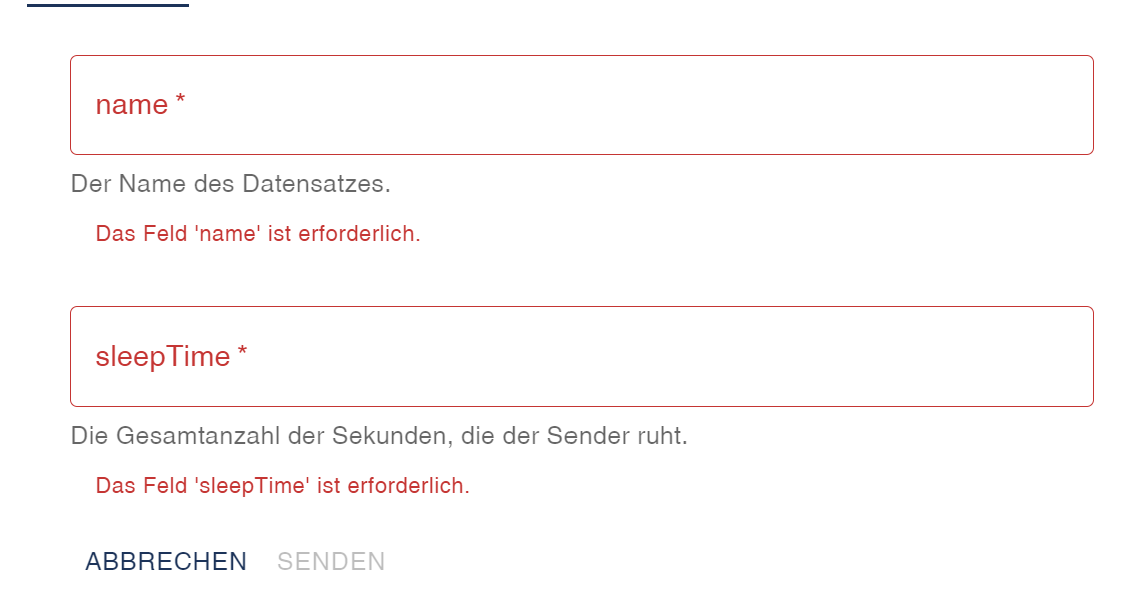
\includegraphics[width=\textwidth]{includes/figures/new_version/rsjf_translation_1.png}
        \caption{Analyse des CGAN tsgm Modells}
        \label{fig:rsjf_translation_1}
    \end{minipage}\hfill
    \begin{minipage}{0.5\textwidth}
        \centering
        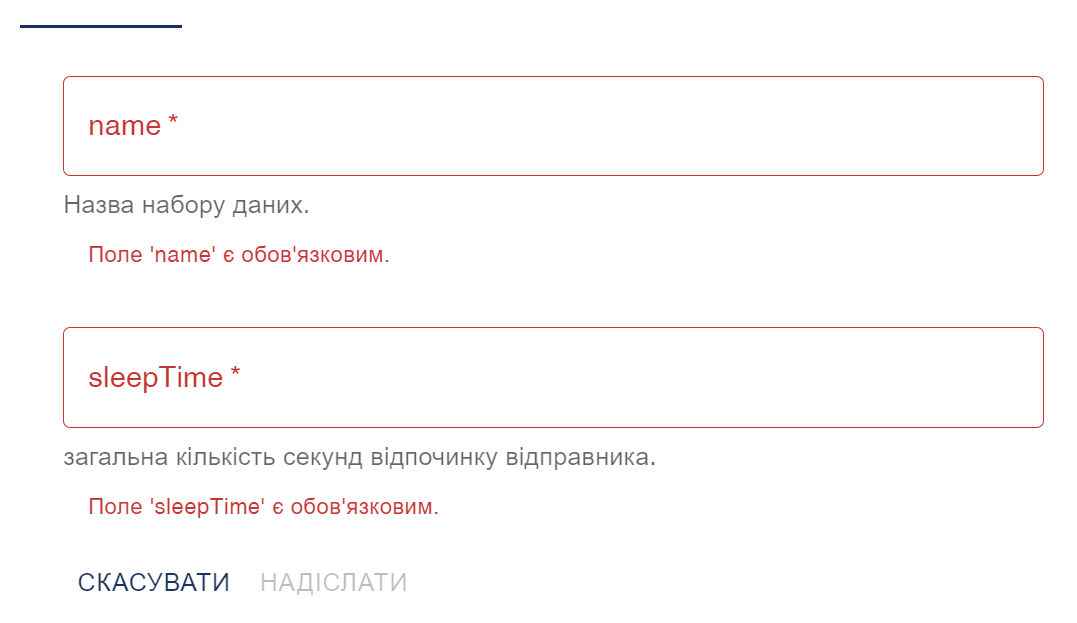
\includegraphics[width=\textwidth]{includes/figures/new_version/rsjf_translation_2.png}
        \caption{Analyse des CGAN Keras Modells}
        \label{fig:rsjf_translation_2}
    \end{minipage}
\end{figure}